\chapter{Results}
\label{chap:results}

This section will provide the results from the data analysis of both parts of the experiment; 1) the agreement regarding the personality traits and characteristics, 2) the AttrakDiff evaluation to assess the user experience. The data was analysed using SPSS.

\section{Part 1 Results: Personality characteristics data analysis}

The characteristics were rated using a scale from 1-5 in which 5 meant a high perceived presence of the characteristic in the interaction with the chatbots, and 1 meant no perceived presence of the characteristics. The data-set was analysed through running a paired-samples t-test, and a two-way repeated measures ANOVA to investigate whether an interaction effect occurred within subjects, as all participants were subjected to all conditions. The analysis performed on this data set will be used to test $H_1 1$: \textit{Users will perceive the personality of Chatbot A as different to the personality of Chatbot B}, $H_1 2$: \textit{Users will perceive the personality of Chatbot A as intended}, and $H_1 3$: \textit{Users will perceive the personality of Chatbot B as intended}. The descriptive statistics of the characteristics data analysis can be found in Table \ref{table:5}.

\begin{table}[h]
\centering
\begin{tabular}{lccccc}
\hline
\multicolumn{6}{c}{\textbf{Descriptive Statistics}} \\
\hline
& N & Minimum & Maximum & Mean & Std. Deviation \\
$Extroversion_A$ & 16 & 2 & 5 & 4,3125 & 0,8116 \\
$Extroversion_B$ & 16 & 1,67 & 3,33 & 2,2708 & 0,47483 \\
$Agreeable_A$ & 16 & 4 & 5 & 4,625 & 0,30277 \\
$Agreeable_B$ & 16 & 2,25 & 4,5 & 3,4219 & 0,57532 \\
$Conscientious_A$ & 16 & 3,33 & 5 & 4,2917 & 0,5146 \\
$Conscientious_B$ & 16 & 2,67 & 4,67 & 3,9167 & 0,60246 \\
$Openness_A$ & 16 & 3 & 5 & 4,0781 & 0,59665 \\
$Openness_B$ & 16 & 1,5 & 5 & 3,4531 & 0,92294 \\
\end{tabular}
 \caption{Descriptive statistics chatbot characteristics results}
 \label{table:5}
    \end{table}

The paired-samples t-test found that there is a significant difference between the two levels of personality and the perceived characteristics. Agreeableness Chatbot B (M=3,4219, SD=,57532) and Agreeableness Chatbot A (M=4,6250, SD=,30277); t(15)=-8,760, p < ,001. Extroversion Chatbot B (M=2,2708, SD=,47483) and Extroversion Chatbot A (M=4,3125, SD=,81166) t(15)=-8,976, p < ,001. Openness Chatbot B (M=3,4531, SD=,92294) and Openness Chatbot A (M=4,0781 SD=,59665) t(15)=-3,727, p = ,002. Conscientiousness Chatbot B (M=3,9167, SD=,60246) and Conscientiousness Chatbot A (M=4,2917, SD=,51460) t(15)=-2,522, p = ,023. These results suggests that participants perceived the two personalities as significantly different from one another. The Mean score difference between Chatbot B and A, suggests that participants perceived all characteristics in Chatbot A to a higher degree than in Chatbot B, where the extroversion factor had the largest difference in mean score.

The two-way repeated measures ANOVA examined whether the starting condition had an interaction effect. The independent variable personality has two levels, and the dependent variable characteristics has four factors where each factor describes a factor from the five factor model (extroversion, agreeable, conscientiousness, openness). The two-way repeated ANOVA included a starting condition (startbot) to investigate whether the order of chatbots participants were subjected to had any effect on the results.

There was a significant main effect of the two levels of personality with respect to the characteristics F(1,14)=73,181, p<,001. There was also a significant main effect between the characteristics F(3,42)=12,960, p<,001. There was an INsignificant interaction effect of the starting condition (personality*characteristics*startbot) p=,380. See Figure \ref{fig:charactmeanAB}.

\begin{figure}[H]
    \centering
    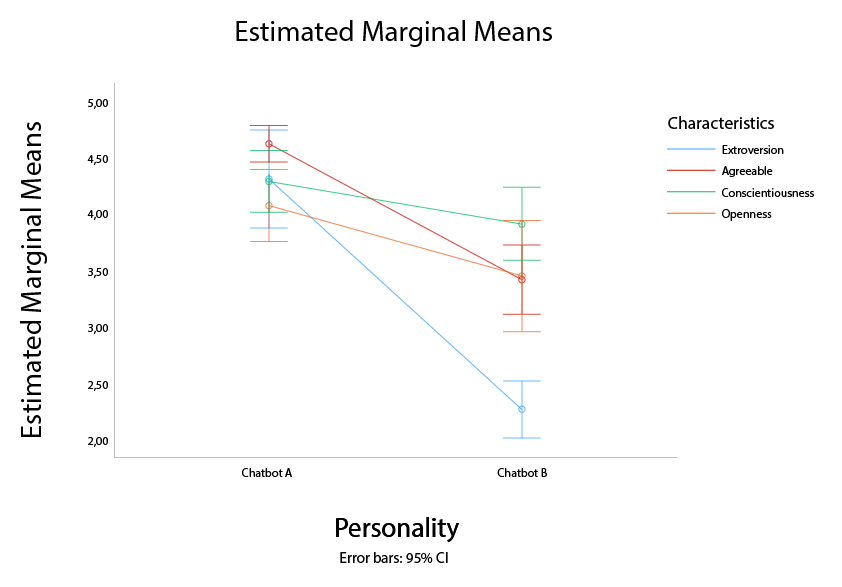
\includegraphics[scale=0.4]{figures/MeansLineCharacteristics.png}
    \caption{Estimated marginal means of characteristics for Chatbot A and Chatbot B}
    \label{fig:charactmeanAB}
\end{figure}

The data was also tested for whether there was an interaction effect of gender. This two-way repeated measures ANOVA revealed no significant interaction effect of gender (Personality*Characteristics*Gender) p=,331. See Figure \ref{fig:perschargender}.

\begin{figure}[H]
    \centering
    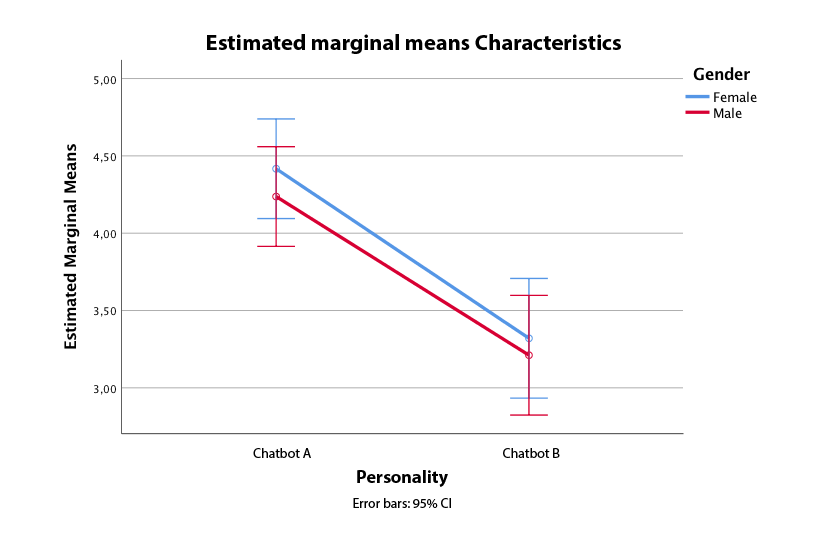
\includegraphics[scale=0.4]{figures/pers-char-gender.png}
    \caption{Estimated marginal means of Chatbot A vs Chatbot B personality on gender}
    \label{fig:perschargender}
\end{figure}

\section{Part 2 Results: AttrakDiff data analysis }
        
The results from the AttrakDiff evaluation was also analysed by running a paired samples t-test, and a two-way ANOVA to understand whether any interaction effects occurred. The statistics will be used to test $H_1 4$: \textit{Personality affects the user experience of chatbots}, and $H_1 5$: \textit{Chatbot A will have an improved effect over Chatbot B}. The descriptive statistics of the AttrakDiff data analysis can be found in Table \ref{table:6}. Descriptive statistic for all word-pairs found in each factor can be found in \ref{desstat}. Personality has two levels (personality, no personality) and user experience has four factors (Pragmatic Quality, Hedonic Quality Stimulation, Hedonic Quality Identity, Attractiveness).

\begin{table}[h]
\centering
\begin{tabular}{lccccc}
\hline
\multicolumn{6}{c}{\textbf{Descriptive Statistics}} \\
\hline
& N & Minimum & Maximum & Mean & Std. Deviation \\
$PQ_A$ & 16 & 4,86 & 6,71 & 5,9286 & 0,56424 \\
$PQ_B$ & 16 & 4 & 6,43 & 5,4732 & 0,5964 \\
$HQ-I_A$ & 16 & 4 & 6,29 & 5,4821 & 0,53165 \\
$HQ-I_B$ & 16 & 3,57 & 5,43 & 4,7679 & 0,56874 \\
$HQ-S_A$ & 16 & 5,14 & 6,14 & 5,625 & 0,29909 \\
$HQ-S_B$ & 16 & 2,57 & 6,57 & 4,7768 & 1,19405 \\
$ATT_A$ & 16 & 5,14 & 7 & 6,3482 & 0,44864 \\
$ATT_B$ & 16 & 3,9 & 6,3 & 5,339 & 0,7805 \\
\end{tabular}
\caption{Descriptive statistics AttrakDiff results}
 \label{table:6}
    \end{table}

The paired samples t-test found that there is a significant difference in the scores between Chatbot B and Chatbot A, where all four factors of the user experience showed a significant improved effect between Chatbot B and A. Pragmatic Quality Chatbot B (M=5,4732, SD=,59649) and Pragmatic Quality Chatbot A (M=5,9286, SD=56424); t(15)=-2,152, p = ,048. Hedonic-I Quality Chatbot B (M=4,7679, SD=,56874) and Hedonic-I Quality Chatbot A (M=5,4821, SD=,53165) t(15)=-3,239, p = ,006. Hedonic-S Quality Chatbot B (M=4,7768, SD=1,19405) and Hedonic-S Quality Chatbot A (M=5,6250 SD=,29909) t(15)=-2,934, p = ,010. Attractiveness Chatbot B (M=5,339, SD=,7805) and Attractiveness Chatbot A (M=6,3482, SD=,44864) t(15)=-4,069, p = ,001. These results suggests that personality has an improved effect on the user experience of chatbots, as all four factors of user experience was scored higher for Chatbot A than Chatbot B. See Figure \ref{fig:meansuxline}

A two-way repeated measures ANOVA was conducted to investigate the effect the starting condition (startbot) had on the independent variable personality and the dependent variable user experience. There was a significant main effect of the two levels of personality with respect to the user experience F(1,14)=15,300, p=,002), and the starting condition (startbot) had no significant interaction effect on personality p=,847. There was a significant main effect of the user experience F(3,42)=12,264, p<,001, and the starting condition (startbot) had no significant interaction effect on user experience p=,865. There was no significant interaction effect between personality, user experience and starting condition (personality*UXscore*startbot) p=,909.

\begin{figure}[H]
    \centering
    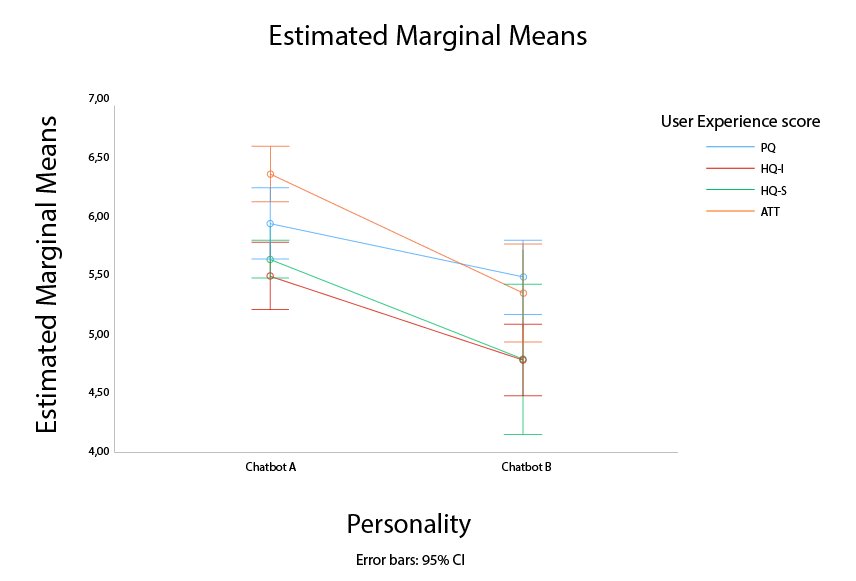
\includegraphics[scale=0.4]{figures/MeansLineUX.png}
    \caption{Estimated marginal means starting condition chatbot A user experience score}
    \label{fig:meansuxline}
\end{figure}

Another two-way repeated measures ANOVA was conducted to investigate whether gender had any significant interaction effect on the variables. The analysis found that there was no significant interaction effect between personality, user experience and gender (personality*UXscore*gender) p=,436.

\begin{figure}[H]
    \centering
    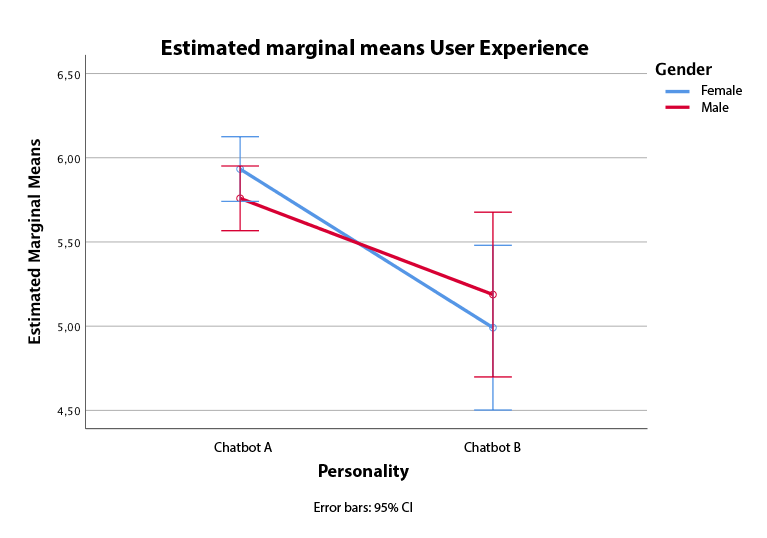
\includegraphics[scale=0.4]{figures/pers-gender.png}
    \caption{Estimated marginal means of Chatbot A and B personalities on gender}
    \label{fig:persgender}
\end{figure}

As shown in Figure \ref{fig:portres}, Chatbot A performed better in both hedonic and pragmatic quality than Chatbot B. The rectangles shows the confidence observed for Chatbot A and B, where Chatbot A has a smaller confidence rectangle implying that the participants were largely at one. Chatbot B however has a much larger confidence rectangle, which suggests that participant responses differed more greatly. Figure \ref{fig:diagval} shows the mean score of each user experience factor and how the two personalities scored compared to each other. The diagram shows that the difference is greater when it comes to hedonic quality-simulation and attractiveness, while the differences are less when it comes to pragmatic quality in particular. As the two personalities only shared traits found in the conscientiousness personality factor (reliable, consistent, perceptive) this result is to be expected as those traits are often found to be pragmatic qualities. Figure \ref{fig:wordpairs} shows the average score for each of the word-pairs for both chatbot versions.

\begin{figure}[h]
    \centering
    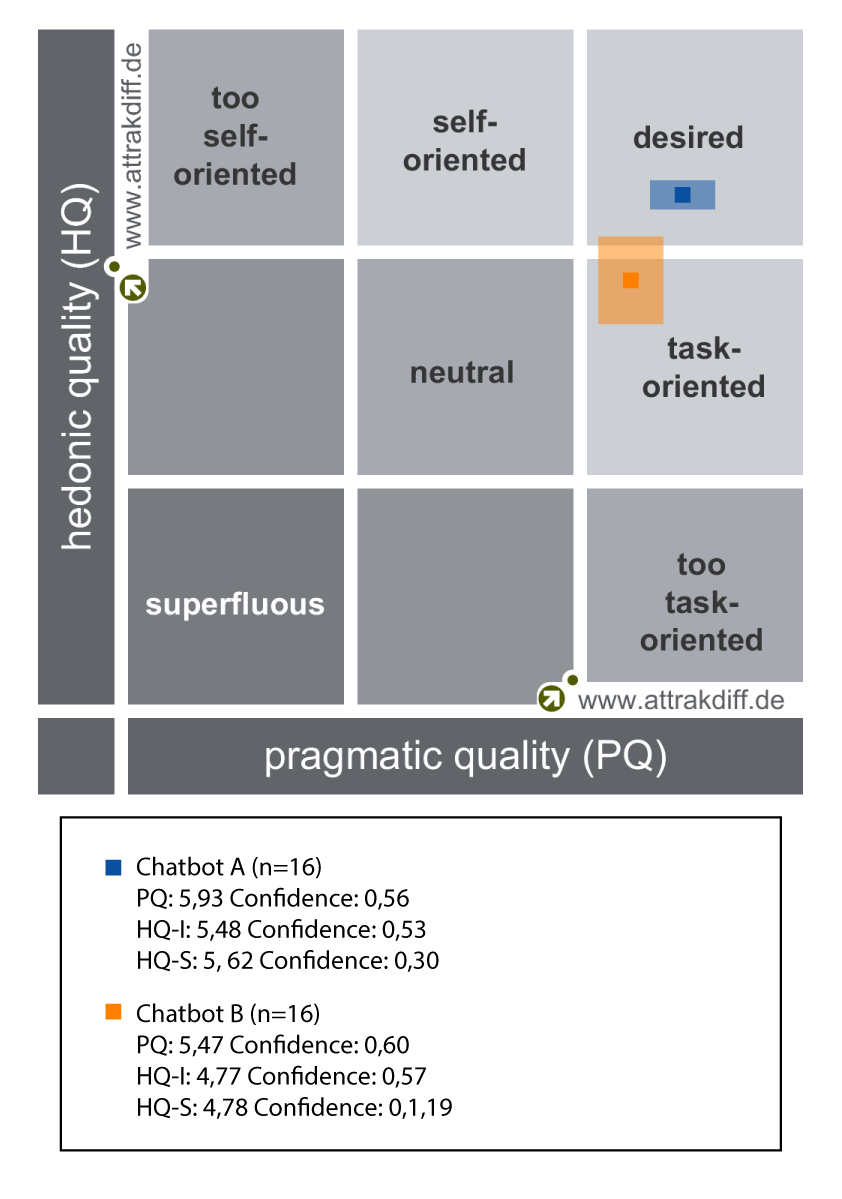
\includegraphics[scale=0.33]{figures/Portfolio-of-results-attrakdiff.png}
    \caption{Results Attrakdiff}
    \label{fig:portres}
\end{figure}

\begin{figure}[h]
    \centering
    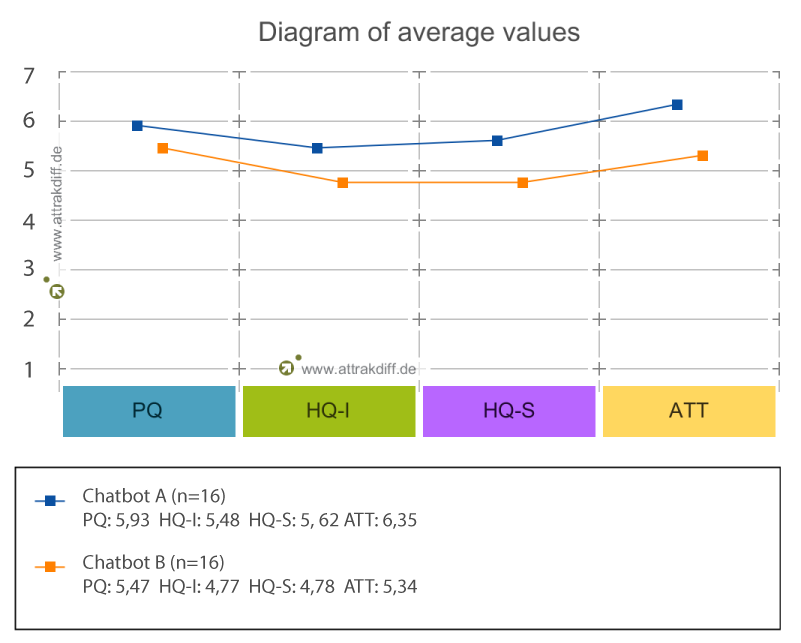
\includegraphics[scale=0.5]{figures/Diagram-of-average-values.png}
    \caption{Diagram of average values}
    \label{fig:diagval}
\end{figure}

\begin{figure}[h]
    \centering
    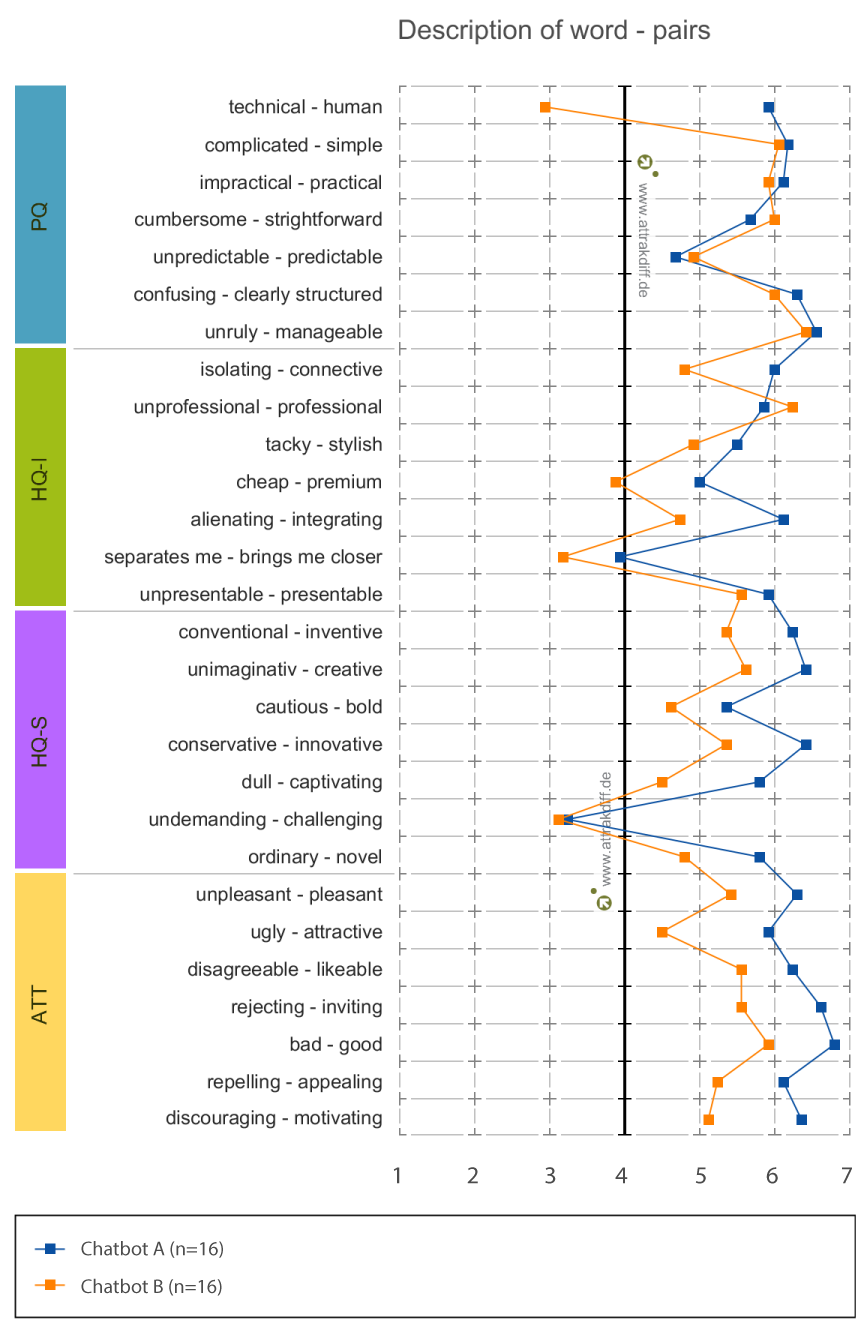
\includegraphics[scale=0.4]{figures/Description-of-word-pairs.png}
    \caption{Description of word-pairs}
    \label{fig:wordpairs}
\end{figure}